\section{Performance on Different Networks}\label{sec:methodology}
We begin by measuring how VCAs perform under different network conditions. 
In the first set of experiments, we study the impact of \textbf{bandwidth}, \textbf{latency}, 
and \textbf{loss} on application performance. In the second set of experiments, 
we analyze how these applications respond to new flows on the network.
\subsection{Static Network Conditions}


\noindent\textbf{Methodology}. 


\begin{figure}[]
    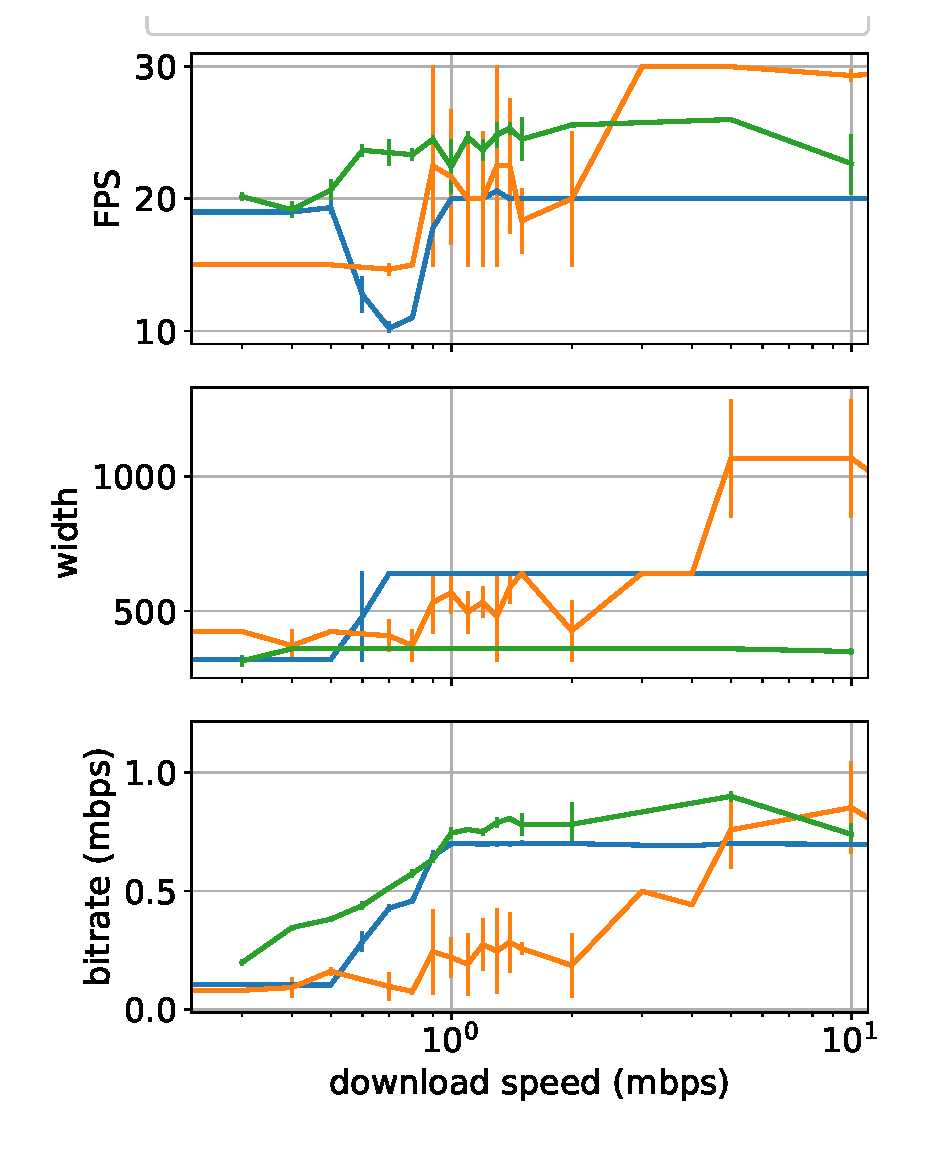
\includegraphics[width=0.35\textwidth,keepaspectratio]{../figures/static/downlink_qos_meet_teams_zoom.eps}
    \caption{Downlink bandwidth and video quality}
	\label{fig:downlink_video_qual}
\end{figure}


\begin{figure}[]
    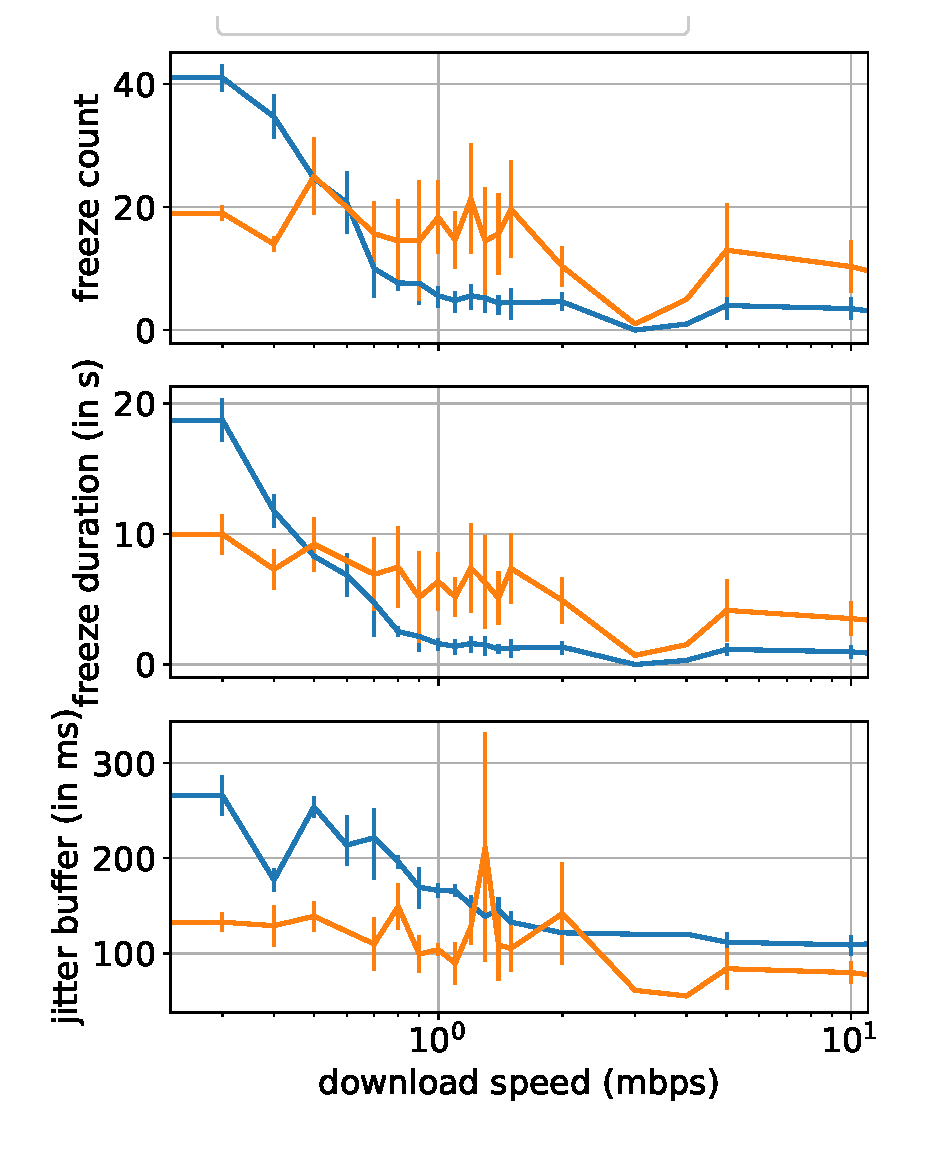
\includegraphics[width=0.35\textwidth,keepaspectratio]{../figures/static/downlink_freeze_meet_teams.eps}
    \caption{Downlink bandwidth and video freezes}
    \label{fig:downlink_freeze}
\end{figure}


\begin{figure}[]
    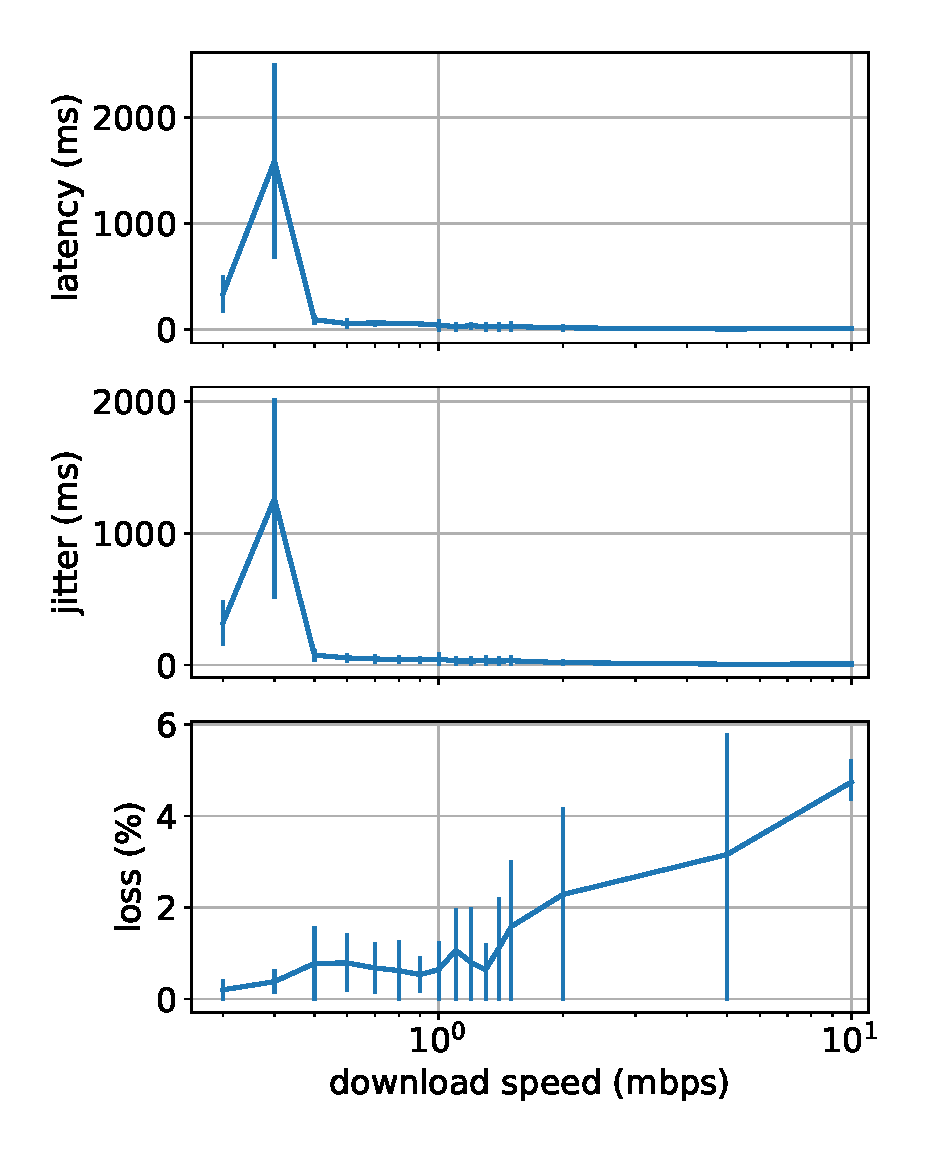
\includegraphics[width=0.35\textwidth,keepaspectratio]{../figures/static/downlink_latency_zoom.eps}
    \caption{Downlink bandwidth and QoS metrics zoom}
    \label{fig:downlink_qos}
\end{figure}


\begin{figure}[]
    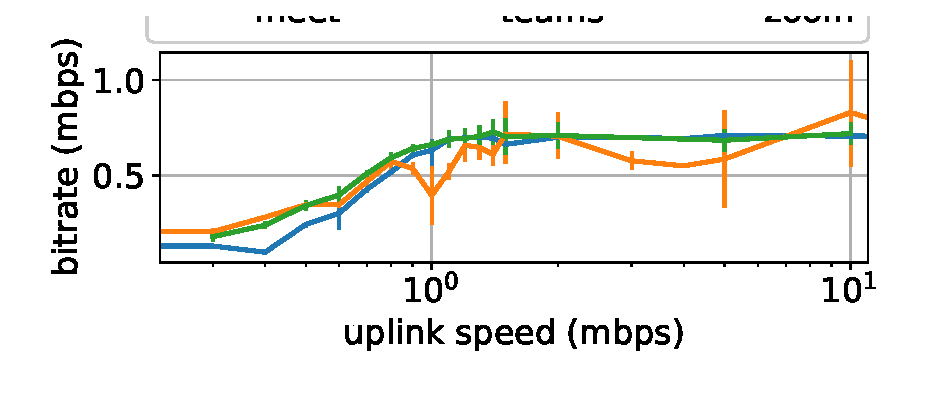
\includegraphics[width=0.35\textwidth,keepaspectratio]{../figures/static/uplink_qos_meet_teams_zoom.eps}
    \caption{Uplink bandwidth and sent video bitrate}
    \label{fig:uplink_bitrate}
\end{figure}


\begin{figure}[]
    \includegraphics[width=0.35\textwidth,keepaspectratio]{../figures/static/uplink_latency_zoom.eps}
    \caption{Uplink bandwidth and QoS metrics}
    \label{fig:uplink_qos}
\end{figure}


\begin{figure}[]
    \includegraphics[width=0.35\textwidth,keepaspectratio]{../figures/static/latency_qos_meet_teams_zoom.eps}
    \caption{Latency and video quality}
    \label{fig:latency_video_qual}
\end{figure}


\begin{figure}[]
    \includegraphics[width=0.35\textwidth,keepaspectratio]{../figures/static/latency_freeze_meet_teams.eps}
    \caption{Latency and video freezes}
    \label{fig:latency_freeze}
\end{figure}


\begin{figure}[]
    \includegraphics[width=0.35\textwidth,keepaspectratio]{../figures/static/latency_latency_zoom.eps}
    \caption{Latency and QoS metrics zoom}
    \label{fig:latency_qos}
\end{figure}


\begin{figure}[]
    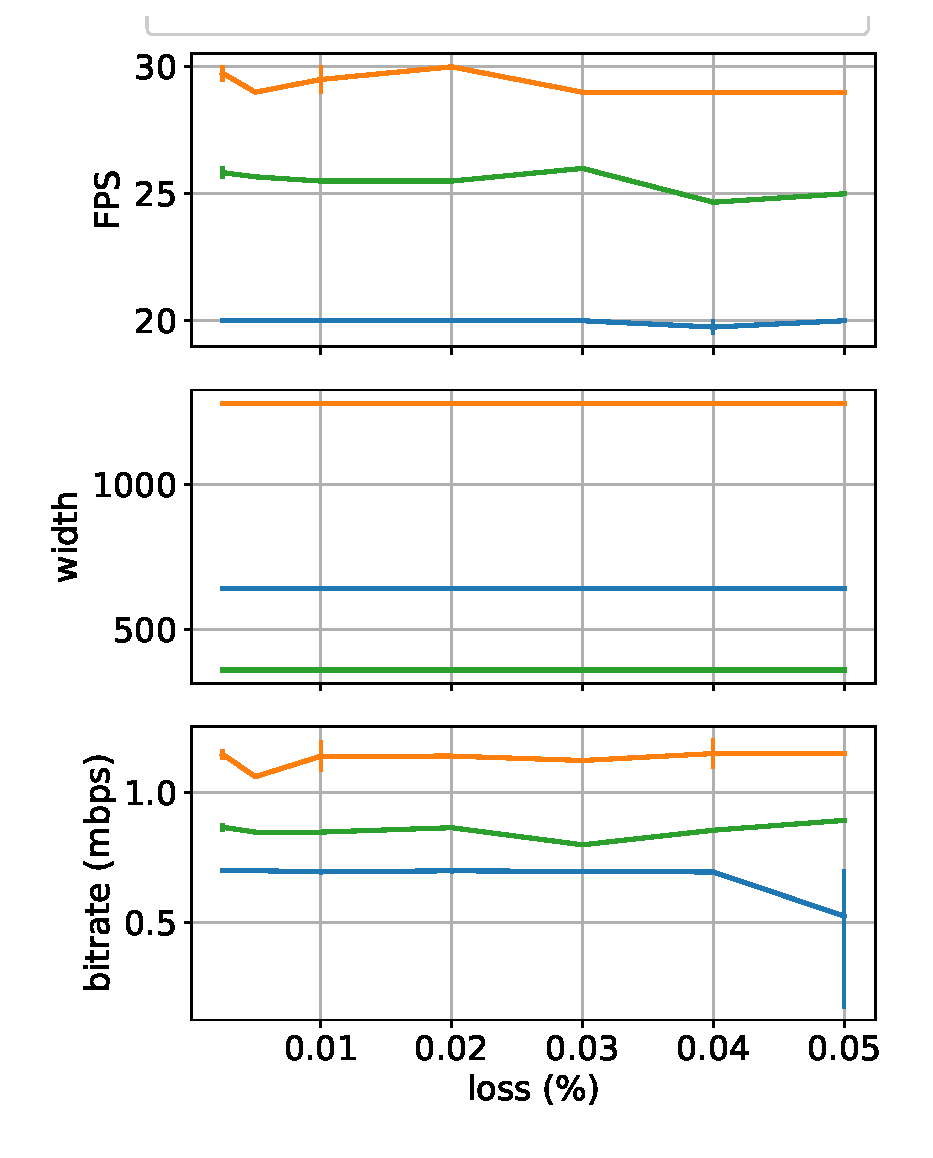
\includegraphics[width=0.35\textwidth,keepaspectratio]{../figures/static/loss_qos_meet_teams_zoom.eps}
    \caption{Loss and video quality}
    \label{fig:loss_video_qual}
\end{figure}


\begin{figure}[]
    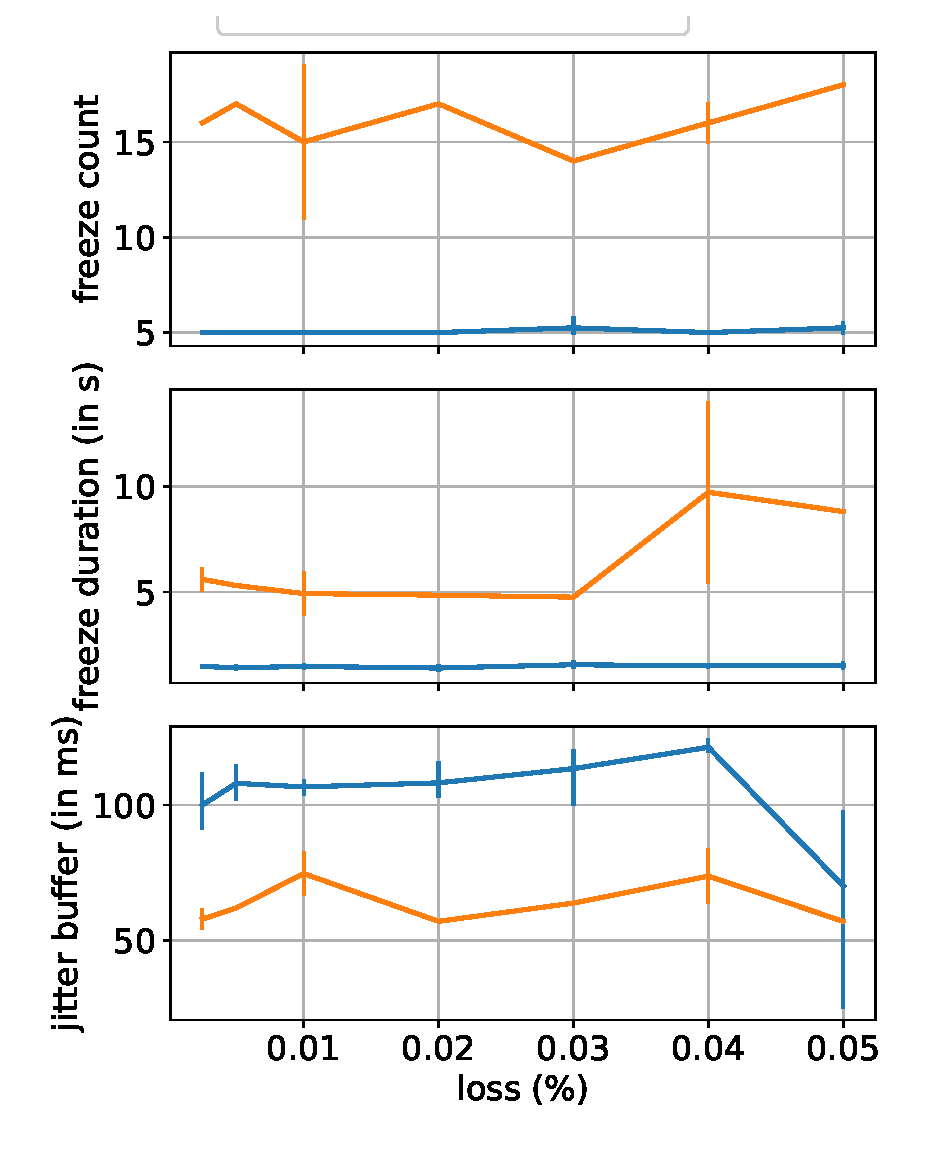
\includegraphics[width=0.35\textwidth,keepaspectratio]{../figures/static/loss_freeze_meet_teams.eps}
    \caption{Loss and video freezes}
    \label{fig:loss_freeze}
\end{figure}


\begin{figure}[]
    \includegraphics[width=0.35\textwidth,keepaspectratio]{../figures/static/loss_latency_zoom.eps}
    \caption{Loss and QoS metrics zoom}
    \label{fig:loss_latency}
\end{figure}


\subsection{Dynamic Network Conditions}

\subsubsection{Temporary Interruptions}

\noindent \textbf{Methodology}.

\subsubsection{Competing Flows}

\noindent \textbf{Methodology}.


